\documentclass[compress]{beamer}
\usepackage{irbookslide}
\usepackage{irilmenau2}
\usepackage{tikz}
\usepackage{url}
\usepackage{ifxetex}
%\RequireXeTeX
\usepackage{fontspec} % zahteva paket euenc
\usepackage{xunicode}
\usepackage{xltxtra}
\usepackage{polyglossia}
\usepackage{minted}
\usepackage{algorithmic}
\renewcommand{\algorithmicrequire}{\textbf{Input:}}
\renewcommand{\algorithmicensure}{\textbf{Output:}}
\usepackage{xcolor,colortbl}
\usepackage{textcomp}
%\setdefaultlanguage[script=Latin]{serbian}

\title{Stabla}
\author{\textcopyright \ \ Goodrich, Tamassia, Goldwasser}
\institute{Katedra za informatiku, Fakultet tehničkih nauka, Univerzitet u
Novom Sadu}
\date{2014.}
\subject{Predavanja sa ASP}

\begin{document}

\frame{\titlepage}

\section[Pojam]{Pojam stabla}
\begin{frame}[fragile]
  \frametitle{Stablo}
  \begin{itemize}
    \item \myred{stablo} je apstraktni model hijerarhijske strukture 
    \item sastoji se od čvorova koji su u vezi \myred{roditelj}/\myred{dete}
    \item svaki čvor ima najviše jednog roditelja; tačno jedan čvor nema roditelja
    \item čvor ima nula ili više dece
  \end{itemize}
  \begin{center}
    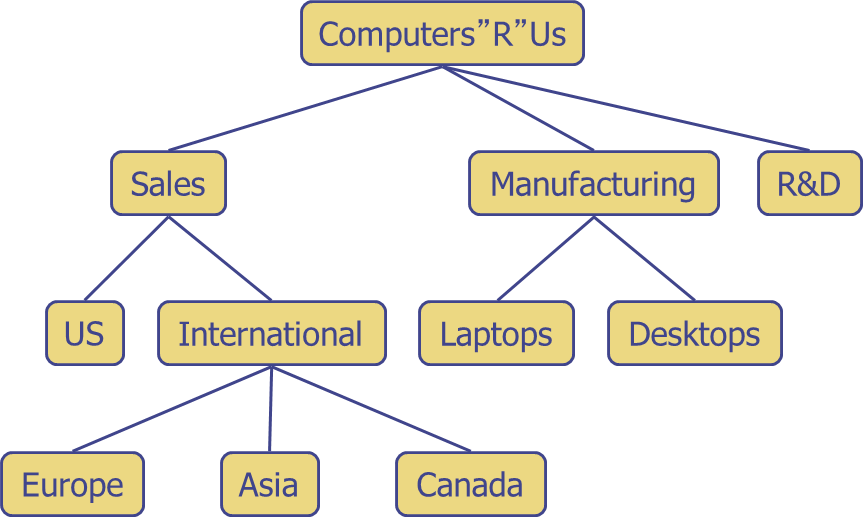
\includegraphics[width=6cm]{asp-08-pic01.png}
  \end{center}
\end{frame}

\begin{frame}[fragile]
  \frametitle{Terminologija}
  \begin{itemize}
    \item \myred{koren} (root): jedini čvor bez roditelja
    \item \myred{unutrašnji čvor}: čvor sa bar jednim detetom
    \item \myred{spoljašnji čvor}/\myred{list} (leaf): čvor bez dece
    \item \myred{predak}: roditelj, deda, pradeda, \ldots do korena
    \item \myred{dubina čvora}: broj predaka
    \item \myred{visina stabla}: najveća dubina
    \item \myred{potomak}: dete, unuče, praunuče, \ldots
    \item \myred{podstablo}: čvor stabla i njegovi potomci
  \end{itemize}
  \begin{center}
    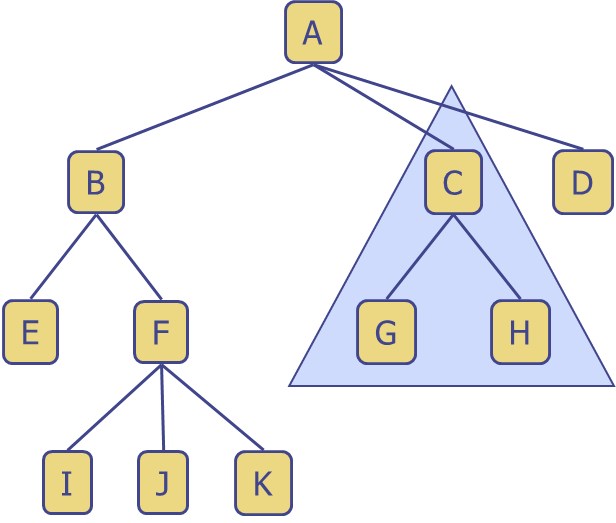
\includegraphics[width=4cm]{asp-08-pic02.png}
  \end{center}
\end{frame}

\begin{frame}[fragile]
  \frametitle{Stablo ATP}
  \begin{itemize}
    \item opšte metode:
    \begin{itemize}
      \item int \myred{len}()
      \item boolean \myred{is\_empty}()
      \item iterator \myred{nodes}()
    \end{itemize}
    \item metode za pristup podacima:
    \begin{itemize}
      \item node \myred{root}()
      \item node \myred{parent}(n)
      \item iterator \myred{children}(n)
      \item int \myred{num\_children}(n)
    \end{itemize}
    \item metode za ispitivanje čvorova:
    \begin{itemize}
      \item boolean \myred{is\_leaf}(n)
      \item boolean \myred{is\_root}(n)
    \end{itemize}
    \item ažuriranje sadržaja:
    \begin{itemize}
      \item element \myred{replace}(n, o)
    \end{itemize}
  \end{itemize}
\end{frame}

\begin{frame}[fragile,shrink]
  \frametitle{Čvor stabla u Pythonu}
\begin{minted}[linenos=false]{python}
class TreeNode:
  def __init__(self):
    self.element = None
    self.parent = None
    self.children = []
  
  def __eq__(self, other):
    return self == other:
    
  def __ne__(self, other):
    return self != other
  
  def is_root(self):
    return self.parent == None
    
  def is_leaf(self):
    return size(self.children) == 0
\end{minted}
\end{frame}

\begin{frame}[fragile,shrink]
  \frametitle{Stablo u Pythonu $_1$}
\begin{minted}[linenos=false]{python}
class Tree:
  def __init__(self):
    self._root = None
  
  def is_empty(self):
    return self._root == None
    
  def depth(self, node):
    if node.parent is None:
      return 0
    else:
      return 1 + self.depth(node.parent)
\end{minted}
\end{frame}

\section[Obilazak]{Obilazak stabla}
\begin{frame}[fragile]
  \frametitle{Obilazak stabla}
  \begin{itemize}
    \item obilazak \myred{po dubini} (depth-first): obiđi čvor i njegove potomke pre braće
    \begin{itemize}
      \item \myred{preorder}: prvo čvor pa deca
      \item \myred{postorder}: prvo deca pa čvor
    \end{itemize}
    \item obilazak \myred{po širini} (breadth-first): obiđi čvor i njegovu braću pre potomaka
    \begin{itemize}
      \item obilazak ,,po generacijama`` u stablu
    \end{itemize}
  \end{itemize}
\end{frame}

\begin{frame}[fragile]
  \frametitle{Obilazak stabla po dubini / preorder}
\myred{preorder}($n$)
\begin{algorithmic}
\STATE obradi($n$)
\FORALL{dete $c$ od $n$}
  \STATE preorder($c$)
\ENDFOR
\end{algorithmic}
\begin{center}
  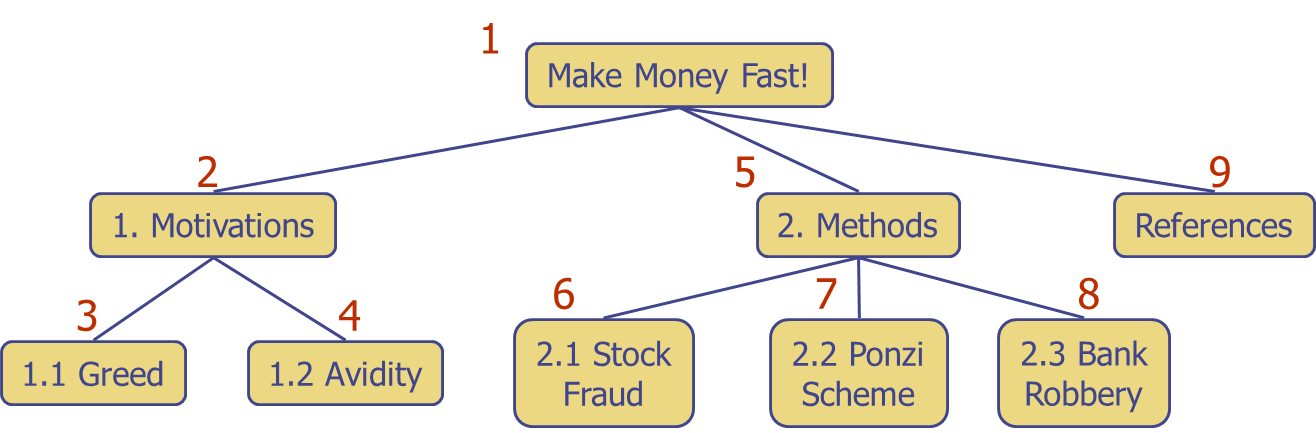
\includegraphics[width=11cm]{asp-08-pic03.png}
\end{center}
\end{frame}

\begin{frame}[fragile]
  \frametitle{Obilazak stabla po dubini / postorder}
\myred{postorder}($n$)
\begin{algorithmic}
\FORALL{dete $c$ od $n$}
  \STATE postorder($c$)
\ENDFOR
\STATE obradi($n$)
\end{algorithmic}
\begin{center}
  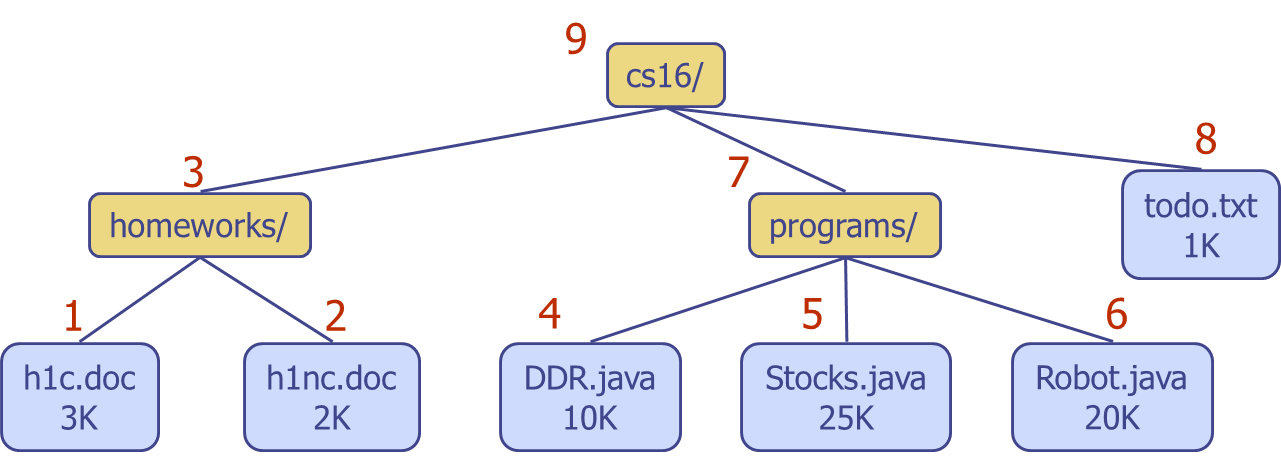
\includegraphics[width=11cm]{asp-08-pic04.png}
\end{center}
\end{frame}

\begin{frame}[fragile,shrink]
  \frametitle{Stablo u Pythonu $_2$}
\begin{minted}[linenos=false]{python}
class Tree:
  ...
  def preorder(self, func):
    self._preorder(self._root, func)
    
  def postorder(self, func):
    self._postorder(self._root, func)
    
  def _preorder(self, node, func):
    func(node)
    for child in node.children:
      self._preorder(child, func)
  
  def _postorder(self, node, func):
    for child in node.children:
      self._postorder(child, func)
    func(node)
\end{minted}
\end{frame}

\begin{frame}[fragile]
\frametitle{Obilazak stabla po širini}
\begin{itemize}
  \item treba obići sve čvorove dubine $d$ pre nego što se pređe na čvorove dubine $d + 1$
  \item primer: stablo igre -- svi mogući ishodi igre koju igra čovek ili računar; koren je početno stanje igre
  \item za igru ,,puta-nula`` (tic-tac-toe)
\end{itemize}
\begin{center}
  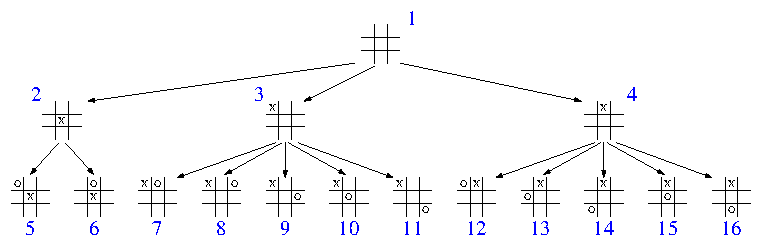
\includegraphics[width=11cm]{asp-08-pic05.pdf}
\end{center}
\end{frame}

\begin{frame}[fragile]
\frametitle{Obilazak stabla po širini}
\begin{columns}
  \begin{column}[c]{6cm}
    \myred{breadth\_first}($root$)
    \begin{algorithmic}
    \STATE napravi novi prazan red $Q$
    \STATE $Q$.add($root$)
    \WHILE{$Q$ nije prazan}
      \STATE $node \leftarrow Q$.dequeue()
      \STATE obradi($node$)
      \FORALL{$child$ dete od $node$}
        \STATE $Q$.enqueue($child$)
      \ENDFOR  
    \ENDWHILE
    \end{algorithmic}
  \end{column}
  \begin{column}[c]{5cm}
    \begin{center}
      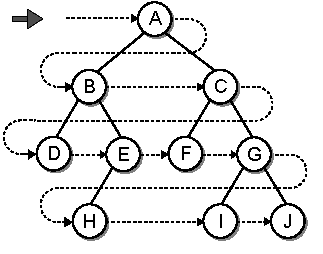
\includegraphics[width=5cm]{asp-08-pic06.pdf}
    \end{center}
  \end{column}
\end{columns}
\end{frame}

\section[2-Stablo]{Binarna stabla}
\begin{frame}[fragile]
  \frametitle{Binarno stablo}
  \begin{itemize}
    \item stablo za koje važi:
    \begin{itemize}
      \item svaki čvor ima najviše dvoje dece
      \item svako dete je označeno kao \myred{levo dete} ili \myred{desno dete}
      \item levo dete po redosledu prethodi desnom detetu 
    \end{itemize}
    \item levo podstablo -- levo dete kao koren
    \item desno podstablo -- desno dete kao koren
    \item \myred{pravilno} binarno stablo: svaki čvor ima 0 ili 2 deteta
  \end{itemize}
  \begin{center}
    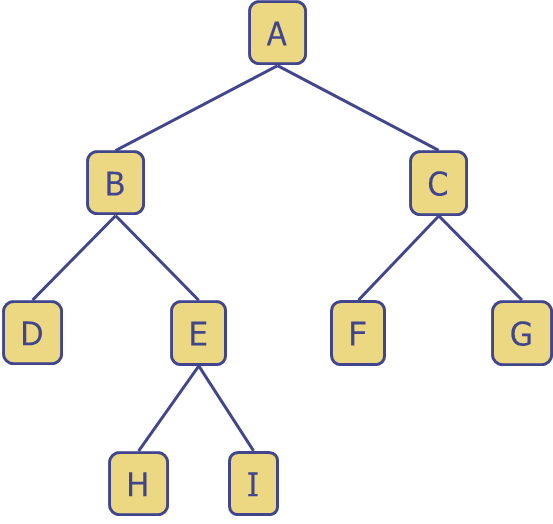
\includegraphics[width=4cm]{asp-08-pic07.png}
  \end{center}
\end{frame}

\begin{frame}[fragile]
  \frametitle{Osobine binarnog stabla}
  \begin{itemize}
    \item nivo stabla $d$ ima najviše $2^d$ čvorova
    \item broj čvorova po nivou raste eksponencijalno
  \end{itemize}
  \begin{center}
    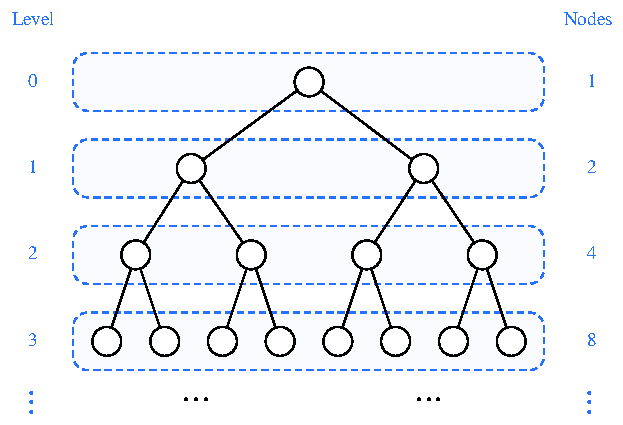
\includegraphics[width=8cm]{asp-08-pic08.pdf}
  \end{center}
\end{frame}

\begin{frame}[fragile]
  \frametitle{Osobine binarnog stabla}
\begin{columns}
  \begin{column}[c]{6cm}
  \begin{itemize}
    \item $n$ -- broj čvorova
    \item $e$ -- broj listova
    \item $i$ -- broj internih čvorova
    \item $h$ -- visina \\ \ \\
    \item $e = i+1$
    \item $n = 2e-1$
    \item $h\leq i$
    \item $h\leq (n-1)/2$
    \item $e\leq 2^h$
    \item $h\geq \log_2 e$
    \item $h\geq log_2(n+1)-1$
  \end{itemize}
  \end{column}
  \begin{column}[c]{5cm}
  \begin{center}
    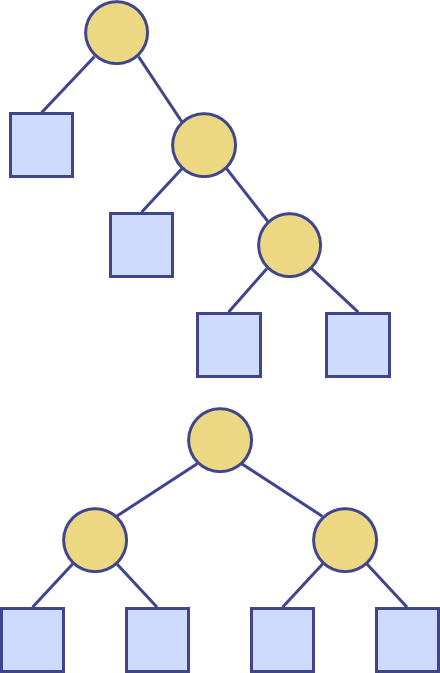
\includegraphics[width=4cm]{asp-08-pic09.png}
  \end{center}
  \end{column}
\end{columns}
\end{frame}

\begin{frame}[fragile]
  \frametitle{Stablo aritmetičkih izraza}
  \begin{itemize}
    \item binarno stablo kreirano na osnovu aritmetičkog izraza
    \item unutrašnji čvorovi -- operatori
    \item listovi -- operandi
    \item primer: $2 * (a - 1) + 3 * b$
  \end{itemize}
  \begin{center}
    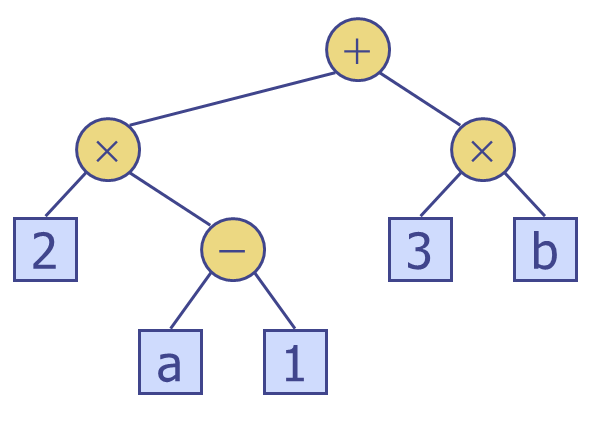
\includegraphics[width=6cm]{asp-08-pic10.png}
  \end{center}
\end{frame}

\end{document}
